\documentclass[letterpaper,12pt]{article}
\usepackage{mathtools}
\DeclarePairedDelimiter\abs{\lvert}{\rvert}     %serve per mettere il modulo 
\usepackage{booktabs}
\usepackage{bm}
\usepackage{textcomp}
\usepackage{colortbl}
\usepackage{tabularx}
\usepackage{textcomp}
\usepackage{siunitx}
\usepackage{booktabs}
\usepackage{enumitem}
\usepackage{xcolor}
\usepackage{fancyhdr}
\usepackage{caption}
\usepackage{changepage}
\usepackage{amsmath} 
\usepackage{subcaption}
\usepackage{graphicx}
\usepackage[table]{xcolor} 
\usepackage[margin=1in,letterpaper]{geometry} % decreases margins
\usepackage{cite} % takes care of citations
\usepackage[hidelinks]{hyperref} % adds hyper links inside the generated pdf file
\usepackage{siunitx} % provides the \SI{}{} command for proper typesetting of units
% Define the colors
\definecolor{linkcolor}{RGB}{0, 102, 204}
\definecolor{citecolor}{RGB}{34, 139, 34}
\definecolor{urlcolor}{RGB}{255, 69, 0}

% Setup hyperref
\hypersetup{
    colorlinks=false, % colored links
    linkcolor=linkcolor, % color for internal links
    citecolor=citecolor, % color for citations
    urlcolor=urlcolor, % color for URLs
}
\fancypagestyle{logoheader}{
    \fancyhf{}
    \fancyhead[L]{
\includegraphics[width = 3cm]{infn-art-science-universita-degli-studi-di-milano-bicocca-maintainer-universita-studi-milano-bicocca.png}}
    \renewcommand{\headrulewidth}{0pt}
    }
\usepackage{blindtext}
\graphicspath{{immagini/}}
%Required for inserting images
%++++++++++++++++++++++++++++++++++++++++
%Margini 



\begin{document}

\title{{\small Università degli studi Milano-Bicocca  Dipartimento di Fisica - Laboratorio II }\\
	Esperienza Ottica - Microonde}
\author{F. Ballo, S. Franceschina, S. Dolci - Gruppo T1 39}
\date{\today}
\maketitle
\thispagestyle{logoheader}


\begin{abstract}
	Nella seguente relazione vengono presentati i risultati ottenuti dalla quarta esperienza del corso di Laboratorio II riguardante l'analisi di fenomeni ottici. L'obiettivo di questa esperienza è quello di studiare le proprietà caratteristiche delle onde elettromagnetiche nello spettro delle microonde. Ci si rifà all'utilizzo di emettitori e ricevitori per registrare il segnale delle onde altrimenti invisibili all'occhio umano (lunghezza d'onda circa 2.85cm).
	\begin{adjustwidth}{-1cm}{-1cm}
	\end{adjustwidth}
\end{abstract}
\tableofcontents
\newpage

\section{Caratteristiche del fascio}

\subsection{Configurazione del circuito e della strumentazione}
Di seguito riportiamo informazioni sulla strumentazione, sulle modalità di misura e in generale gli obiettivi di questa esperienza.
Per studiare i vari fenomeni e le proprietà ottiche di onde elettromagnetiche abbiamo utilizzato come strumentazione 
quella fornita da PASCO scientific "Advanced Microwave Optics System , WA-9316A".
Di seguito abbiamo allegato un manuale che contiene tutte le informazioni riguardo alla
\href{https://cdn.pasco.com/product_document/Microwave-Optics-Experiment-Guide-WA-9314C.pdf}{strumentazione (clicca qui)}.
Per quanto riguarda i fasci utilizzati, un diodo Gunn fa da sorgente di microonde linearmente polarizzate con lunghezza d'onda pari a $2.85$cm. Per la presa di misure un multimetro palmare è stato collegato al ricevitore, dunqe l'intensità del segnale è stata misurata registrando la $\Delta V$, mentre per quanto riguarda la misura di angoli abbiamo utilizzato un goniometro graduato.
\
\subsection{Polarizzazione}
\paragraph*{Legge di Malus}
Il primo obbiettivo dell'esperienza è stato quello di caratterizzare il fascio di microonde emesso dall'emettitore.
Per fare ciò, abbiamo cominciato verificando la direzione di polarizzazione del fascio. \\
Abbiamo posizionato l'emettitore e il ricevitore uno di fronte all'altro, in modo che fossero
allineati ed a una distanza fissa. Abbiamo quindi ruotato gradualmente il ricevitore e campionato
la tensione rilevata dal ricevitore, fino ad aver compiuto una rotazione di 180 gradi.\\
Dal manuale Pasco sappiamo che l'emettitore emette un fascio coerente polarizzato linearmente
e il ricevitore è sensibile solo ad una certa polarizzazione. Il comportamento che ci aspettiamo
di osservare da questo esperimento è quello previsto dalla legge di Malus:
\begin{equation}
	I = I_0 \cos^2(\theta)
	\label{eq:malus}
\end{equation}
Dove $I_0$ è l'intensità massima e $\theta$ è l'angolo tra la direzione di polarizzazione del fascio e quella rilevata dal ricevitore.\\
Abbiamo rappresentato i dati raccolti in figura \ref{fig:polarizzazione} e sovrapposti alla legge di Malus \eqref{eq:malus}.
Infine, abbiamo calcolato il valore del $\tilde{\chi^2} = 12.7$.


\begin{figure}[h!]
	\centering
	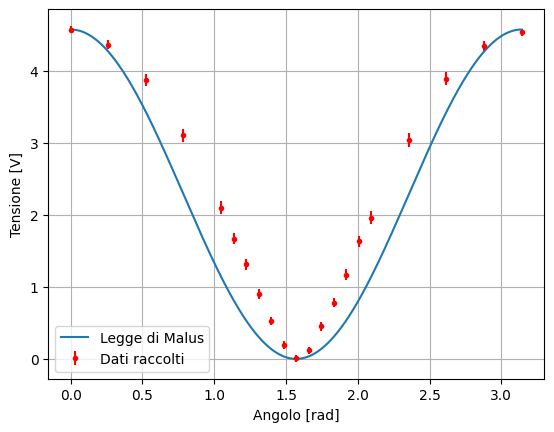
\includegraphics[width = 0.7\textwidth]{polarizzazione.png}
	\caption{Intensità del segnale rilevato in funzione dell'angolo di rotazione}
	\label{fig:polarizzazione}
\end{figure}

\paragraph*{Filtro polarizzatore}
Applicando un filtro polarizzatore tra emettitore e ricevitore, siamo stati in grado di studiare il cambiamento della lettura del segnale.
Il filtro permetteva il passaggio delle onde polarizzate parallelamente alla sua direzione, e bloccava quelle perpendicolari.\\
Posizionandolo quando gli horn si trovavano orientati a 90 gradi uno rispetto all'altro, non abbiamo osservato alcun cambiamento nella lettura del segnale. 
Questo poiché il ricevitore agiva contemporaneamente da filtro, e con uno sfasamento di $\frac{\pi}{2}$ la lettura era già nulla; dunque la
selezione della direzione di polarizzazione dovuta al filtro non aveva effetto.\\
Quando invece gli horn erano allineati, il filtro polarizzatore aveva la capacità di bloccare il segnale a seconda della rotazione, dunque il ricevitore
rilevava un segnale ridotto o nullo.


\subsection{Ampiezza}
\subsubsection{Intensità in funzione dell'angolo di rotazione}

\begin{figure}[h!]
    \centering
    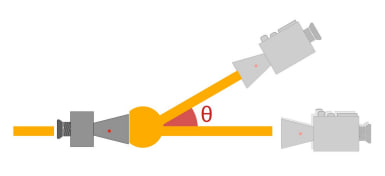
\includegraphics[width = 0.4\textwidth]{ampiezza rotazione.jpg}
    \caption{Impostazione dell'apparato per la misura dell'ampiezza del segnale in funzione dell'angolo di rotazione}
    \label{fig:ampiezza_angolo}
\end{figure}
\newpage

Dopo aver concluso che il rilevatore reagisce all'intensità del segnale, ci siamo dedicati allo studio della geometria
del fascio emesso. Per prima cosa, abbiamo studiato la variazione dell'intensità rilevata al variare dell'angolo di rotazione
tra emettitore e ricevitore.\\
Per fare ciò, abbiamo fissato una distanza tra i due dispositivi e ruotato gradualmente il ricevitore attorno ad un asse
passante di fronte all'emettitore. Abbiamo poi campionato la tensione rilevata dal ricevitore ad intervalli di 5 gradi, fino a quando
il valore misurato è calato a circa zero.\\
Riportiamo i dati raccolti in figura \ref{fig:rotazione}.\\

\begin{figure}[h]
    \centering
    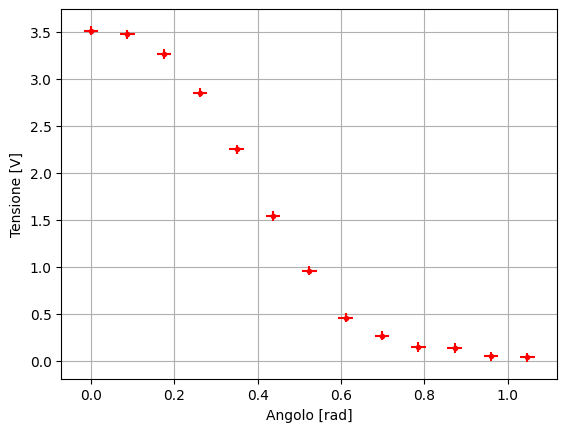
\includegraphics[width = 0.6\textwidth]{dati_rotazione.png}
    \caption{Intensità del segnale rilevato in funzione dell'angolo di rotazione}
    \label{fig:rotazione}
\end{figure}

Per stabilire quale modello stessero seguendo i dati, abbiamo scelto di interpolarli prima con le seguenti funzioni:
\begin{align*}
    & I = I_0\cos(Bx)^A \\
    & I = A\cdot\cos(Bx + C) + D \\
    & I = A\cdot cos(B\theta)^D
\end{align*} 
I risultati dell'interpolazione sono riportati in figura \ref{fig:fit_rotazione}.

\begin{figure}[h!]
    \centering
    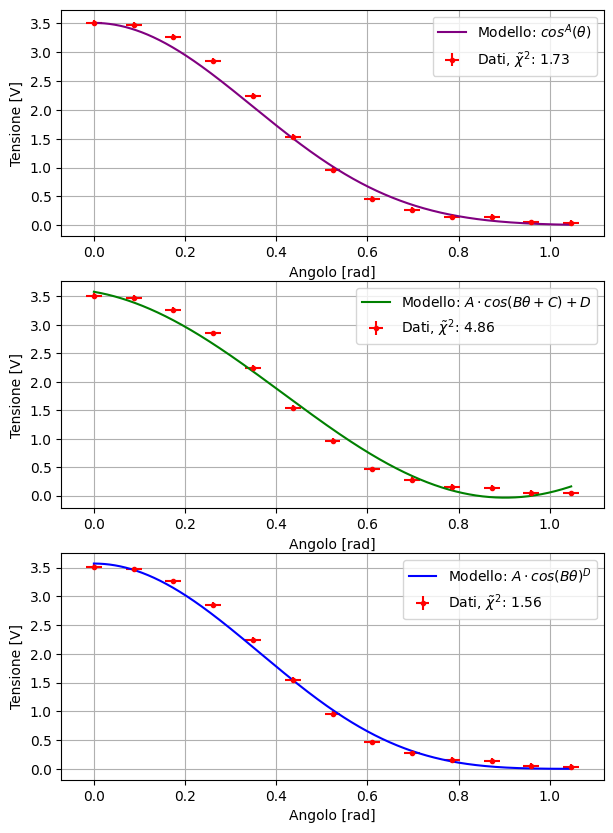
\includegraphics[width = 0.7\textwidth]{fit_rotazione.png}
    \caption{Fit dell'intensità del segnale rilevato in funzione dell'angolo di rotazione}
    \label{fig:fit_rotazione}
\end{figure}

\newpage
\textbf{MANCANO I DATI DEI FIT}
\subsubsection{Intensità in funzione della distanza}
\begin{figure}[h!]
    \centering
    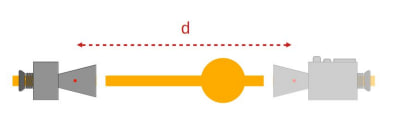
\includegraphics[width = 0.45\textwidth]{ampiezza distanza.jpg}
    \caption{Impostazione dell'apparato per la misura dell'ampiezza del segnale in funzione della distanza tra emettitore e ricevitore}
    \label{fig:ampiezza_distanza}
\end{figure}

Il punto successivo consisteva nello studiare l'andamento dell'intensità del segnale in funzione della distanza tra i
dispositivi. Mantenendo l'emettitore e il ricevitore allineati, abbiamo variato la distanza tra i due
e campionato a intervalli regolari la tensione misurata.\\
A causa del fatto che emettitore e ricevitore si trovavano uno di fronte all'altro, oltre alla decrescita
del segnale dovuta alla distanza, abbiamo osservato un andamento oscillatorio. Questo è dovuto al fatto che
parte del segnale inviato non viene assorbita dal rilevatore, ma viene riflessa e ritorna verso l'emettitore,
che a sua volta riflette parte del segnale. Si forma quindi un'onda stazionaria tra i due dispositivi,
la cui interferenza porta a un andamento oscillatorio dell'intensità osservata.\\
Per cominciare abbiamo campionato ogni 1 cm, per analizzare l'andamento generale del fascio; successivamente,
ci siamo ristretti attorno ad alcuni massimi e misurato con passi di 0.2 cm per farci un idea migliore della forma precisa del segnale.\\

\begin{figure}[h!]
	\centering
	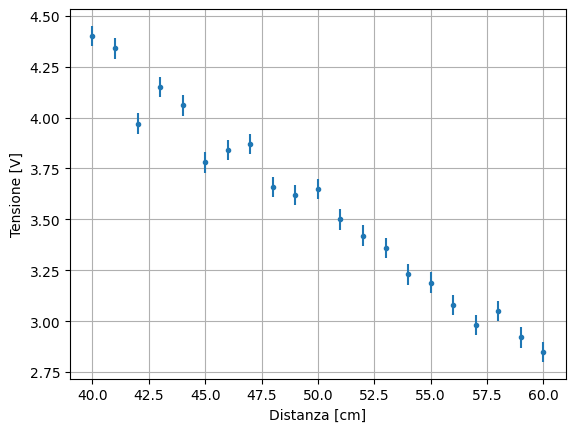
\includegraphics[width = 0.6\textwidth]{dati_distanza.png}
	\caption{Intensità del segnale rilevato in funzione della distanza}
	\label{fig:distanza}
\end{figure}

\paragraph*{Andamento globale del segnale}
Se il fascio si comportasse come un'onda piana ideale, ci aspetteremmo che la sua intensità non dipendesse dalla distanza.
Se invece si comportasse come un'onda sferica, l'andamento dell'intensità dovrebbe essere inversamente proporzionale
al quadrato della distanza. Nella realtà, il segnale avrà un andamento più complesso che non si adatterà perfettamente
a nessuna delle due funzioni.\\
Per capire quale fosse l'andamento dell'intensità del segnale, abbiamo deciso di eseguire un'interpolazione con diverse funzioni,
per vedere quale fosse la più adatta.\\

\begin{figure}[h!]
	\centering
	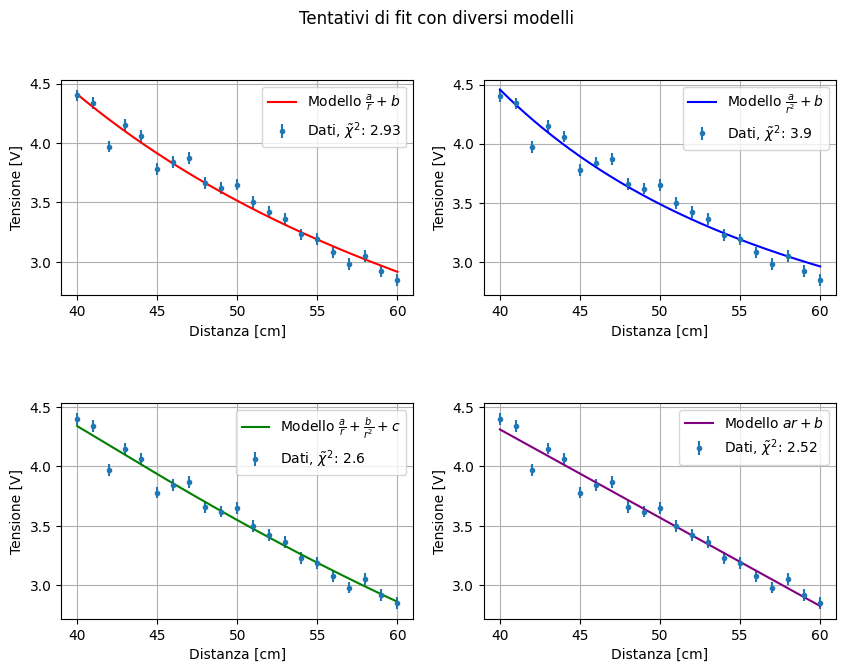
\includegraphics[width = \textwidth]{fit_distanza_vari_modelli.png}
	\caption{Fit dell'intensità del segnale rilevato in funzione della distanza secondo diversi modelli}
	\label{fig:fit_distanza_vari_modelli}
\end{figure}

Non avendo una risoluzione sufficiente per distinguere con precisione massimi e minimi, abbiamo deciso di interpolare
i dati con funzioni non oscillanti. Per giustificare questa scelta, abbiamo considerato il fatto che le oscillazioni dovute all'interferenza
variano attorno ad un valore medio, e che i contributi dovuti ad ogni particolare oscillazione in media si annullano a vicenda.\\
Osservando i grafici in figura \ref{fig:fit_distanza_vari_modelli}, si evince che tra quelli considerati in precedenza, il modello che meglio si adatta
ai dati è quello composito, che considera un adattamento inversamente proporzionale sia al raggio, sia al quadrato di esso.\\
Ci aspettavamo un risultato simile, dal momento che il segnale emesso non è perfettamente né un'onda piana, né una sferica. Peculiare invece,
è il fatto che avendo provato un fit con modello lineare, esso sia quello che ottiene il valore di $\tilde{\chi^2}$ minore. Questo potrebbe essere dovuto al fatto
che sulla scala da noi scelta per le misure, l'andamento del segnale è approssimabile con una retta.\\
Per questo motivo, nella successiva analisi abbiamo deciso di utilizzare il modello lineare per semplicità.\\


\paragraph*{Andamento attorno ai massimi}
Successivamente, abbiamo ricavando la lunghezza d'onda del fascio dai dati campionati più frequentemente, con un passo minore, riportandoli in figura \ref{fig:distanza_zoom}.

\begin{figure}[h!]
	\centering
	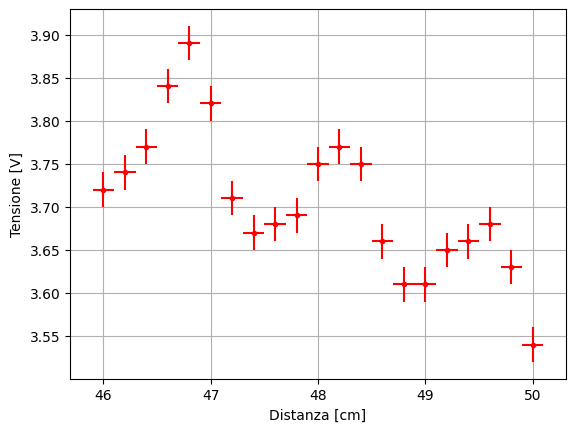
\includegraphics[width = 0.7\textwidth]{dati_distanza_ondulatori.png}
	\caption{Intensità del segnale rilevato in funzione della distanza - zoom attorno ad alcuni massimi}
	\label{fig:distanza_zoom}
\end{figure}

Avendo stabilito che l'andamento dell'intensità del segnale era lineare, abbiamo deciso di interpolare i dati con una funzione del tipo:
\begin{equation}
	I = Ax + B\ + Csin(Dx + E)
	\label{eq:modello_oscillante}
\end{equation}
che corrisponde ad una retta con un'onda sinusoidale sovrapposta.\\
Il risultato del fit è riportato in figura \ref{fig:fit_distanza_ondulatori}.

\begin{figure}[h!]
	\centering
	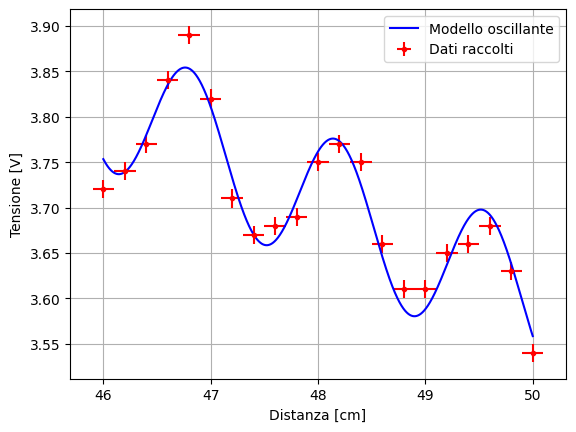
\includegraphics[width = 0.7\textwidth]{fit_distanza_ondulatori.png}
	\caption{Fit dell'intensità del segnale rilevato in funzione della distanza campionato più frequentemente}
	\label{fig:fit_distanza_ondulatori}
\end{figure}

Il fit ha restituito i seguenti valori:
\begin{table}[h!]
	\centering
	\begin{tabular}{|c c|}
		\hline
		\textbf{Parametro} & \textbf{Valore} \\
		\hline
		$A$ & $-0.057 \pm 0.004$ \\
		$B$ & $6.43 \pm 0.18$ \\
		$C$ & $0.077 \pm 0.006$ \\
		$D$ & $4.56 \pm 0.06$ \\
		$E$ & $-67.5 \pm 3.1$ \\
		$\tilde\chi^2$ & $1.1$ \\
		\hline
	\end{tabular}
	\caption{Risultati del fit del modello oscillante}
	\label{tab:fit_distanza_ondulatori}
\end{table}

In questo caso il valore $D$ rappresenta il numero d'onda, quindi la lunghezza d'onda è data da
$$\lambda = 2\cdot \frac{2\pi}{D}$$
dove il fattore 2 sta ad indicare il fatto che la lunghezza d'onda del fascio emesso è il doppio della lunghezza d'onda del segnale che interferisce.\\
Inserendo i valori ottenuti dal fit, propagando l'errore ed eseguendo un test di compatibilità, otteniamo:

\begin{align*}
	 & \lambda = (2.75 \pm 0.04)\ \text{m} \\
	 & \text{compatibilità}: 2.47
\end{align*}

\subsection{Conclusioni}

L'obbiettivo di questa sezione era quello di caratterizzare il fascio di microonde emesso dall'emettitore.\\
Per cominciare, ci siamo domandati la validità della legge di Malus. Osservando il valore del $\tilde{\chi^2}$
ottenuto e il grafico in figura \ref{fig:polarizzazione}, si evince che i dati raccolti non sono compatibili con tale modello.
Tuttavia, dall'analisi dei punti successivi ci siamo convinti che il segnale sia descritto da una funzione più complessa,
non approssimabile con la legge di Malus.\\
In seguito abbiamo tentato di stabilire la geometria del segnale, studiandone l'andamento dell'intensità al variare
dell'angolo di rotazione e della distanza. Da queste misurazioni emerge che il segnale non è né un'onda piana, né sferica,
ma un'onda complessa, 


\section{Angolo di Brewster}
In questa sezione abbiamo studiato il raggio trasmesso e riflesso da una lastra di polietilene al fine di 
determinare l'angolo di Brewster. Come confronto, abbiamo calcolato l'angolo atteso, 
dato dalla formula \ref{eq:brew_atteso}
\begin{equation}
	\theta_B = \arctan\left(\frac{n_2}{n_1}\right)
	\label{eq:brew_atteso}
\end{equation}

Dove $n_1$ = 1.0003 è l'indice di rifrazione dell'aria e $n_2$ = 1.5 è l'indice di rifrazione del polietilene.\\

Per l'analisi del raggio trasmesso abbiamo posto il ricevitore di fronte al trasmettitore, frapponendo la lastra
fra i due. Abbiamo montato la lastra sopra un supporto rotante e 
sistemato l'emettitore in modo che la polarizzazione fosse parallela all'angolo di incidenza. 
Variando l'angolo di incidenza del raggio abbiamo campionato l'intensità del raggio trasmesso.
Per individuare l'angolo di Brewster abbiamo interpolato il picco ottenuto dal grafico con una parabola, di
cui riportiamo il modello:
\begin{equation}
	y = a(x-b)^2 + c
	\label{eq:parabola}
\end{equation}
\\

Per verificare che l'intensità del raggio trasmesso sia dipendente dalla polarizzazione abbiamo
eseguito la stessa procedura per polarizzazione perpendicolare al piano di incidenza,
ruotando l'emettitore di 90 gradi. \\

Per l'analisi del raggio riflesso abbiamo configurato l'apparato in modo tale da far variare sia l'angolo della 
lastra, sia l'angolo tra emettitore e ricevitore, in modo che il ricevitore seguisse il raggio riflesso. Abbiamo 
così campionato l'intensità del raggio riflesso al variare dell'angolo di incidenza.\\

\subsection{Analisi dati}

Utilizzando la formula \ref{eq:brew_atteso} abbiamo calcolato l'angolo di Brewster atteso, 
ottenendo $\theta_B = 56.3$ gradi.\\

Riportiamo di seguito il grafico dell'intensità del raggio trasmesso in funzione dell'angolo di incidenza.\\
\begin{figure}[h!]
	\centering
	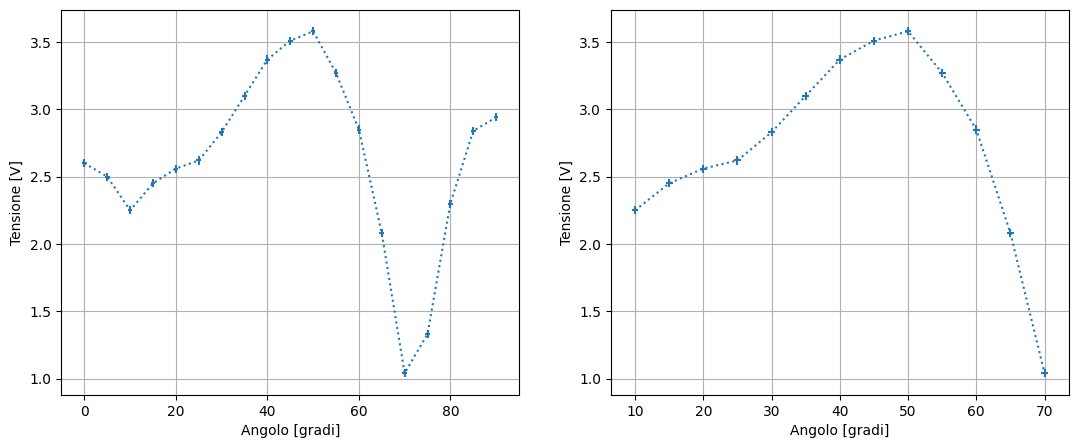
\includegraphics[width = 0.8\textwidth]{trasmesso.png}
	\caption{Intensità del raggio trasmesso in funzione dell'angolo di incidenza}
	\label{fig:trasmesso}
\end{figure}

Abbiamo inserito il grafico con tutte le misurazioni effettuate (grafico di sinistra). Analizzando la figura ci
siamo accorti che l'intensità torna ad aumentare oltre 70 gradi. Questo è dovuto al fatto che la lastra, non 
essendo abbastanza lunga, lasciava passare parte del raggio incidente, determinando un aumento dell'intensità. 
Abbiamo quindi deciso di riportare nel grafico di destra gli unici dati rilevanti per determinare l'angolo di Brewster.\\
Una volta individuata la regione in cui l'intensità aumentava, abbiamo interpolato il picco con un modello parabolico.
Di seguito riportiamo i risultati del fit: 

\begin{figure}[h!]
	\centering
	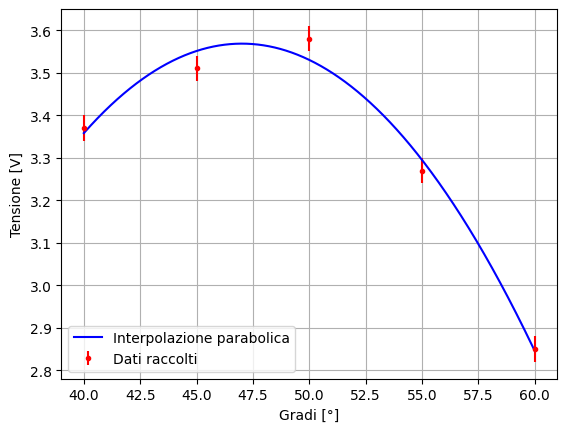
\includegraphics[width = 0.8\textwidth]{brew_angle.png}
	\caption{Interpolazione del picco con modello parabolico}
	\label{fig:parabola}
\end{figure}

\begin{enumerate}
	\item $a = \num{-4.4e-3}  \pm \num{0.5e-3}$
	\item $b = 47.2 \pm 0.4$
	\item $c = 3.57 \pm 0.02$
	\item $\chi^2 = 2.2$
\end{enumerate}

Il parametro b, essendo la traslazione della parabola sull'asse x, rappresenta l'angolo di Brewster. Abbiamo
confrontato l'angolo ottenuto con l'angolo atteso, ottenendo una distanza in deviazioni standard di: 114\\

Riportiamo in figura \ref{fig:wrong_pol} il grafico dell'intensità del raggio trasmesso per la polarizzazione
perpendicolare alla lastra. Abbiamo escluso le ultime misure per lo stesso motivo dell'analisi di raggio trasmesso
con polarizzazione parallela.

\begin{figure}[h]
	\centering
	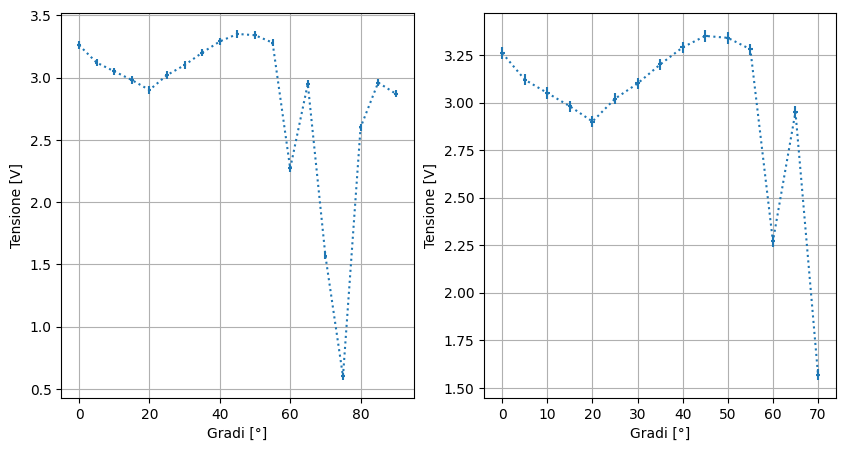
\includegraphics[width = 0.8\textwidth]{wrong_pol.png}
	\caption{Intensità del raggio trasmesso - polarizzazione perpendicolare}
	\label{fig:wrong_pol}
\end{figure}

Nonostante non sia necessario interpolare questa sezione, poichè per polarizzazione perpendicolare non si dovrebbe 
osservare un picco di intensità attorno all'angolo di Brewster, abbiamo deciso di farlo per motivazioni che
saranno spiegate nelle conclusioni. In figura \ref{fig:wrong_pol_fit} riportiamo il grafico dell'interpolazione 
parabolica eseguito attorno all'angolo ottenuto con polarizzazione parallela.

\begin{figure}[h]
	\centering
	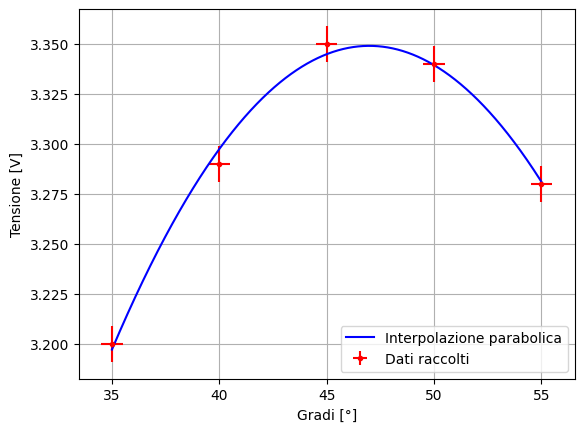
\includegraphics[width = 0.8\textwidth]{wrong_pol_fit.png}
	\caption{Interpolazione del picco con modello parabolico - polarizzazione perpendicolare}
	\label{fig:wrong_pol_fit}
\end{figure}

Di seguito riportiamo i risultati del fit:
\begin{enumerate}
	\item $a = \num{-1.1e-3}  \pm \num{0.3e-3}$
	\item $b = 47 \pm 1$
	\item $c = 3.35 \pm 0.02$
	\item $\chi^2 = 0.1$
\end{enumerate}

\newpage

Per quanto riguarda i dati e i grafici relativi all'intensità del raggio riflesso, li riportiamo in fondo alla 
relazione. Il loro comportamento anomalo li ha resi poco utili per la ricerca dell'angolo di Brewster.
Avendo osservato ciò nella prima giornata di laboratorio, abbiamo effettuato nuovamente le stesse misure 
nella seconda giornata, ma senza ottenere miglioramenti. L'andamento globale dei grafici richiama quello corretto,
ma i numerosi picchi fanno intuire la necessità di un campionamento maggiore.\\

\subsection{Conclusioni}
\paragraph*{Raggio trasmesso} L'andamento dei grafici è in accordo con quanto atteso, perchè osserviamo
un'aumento dell'intensità nell'intorno dei 50 gradi sia per polarizzazione parallela che perpendicolare.
In ogni caso, l'interpolazione parabolica restituisce un valore dell'angolo di Brewster molto distante 
da quello atteso. Abbiamo pensato che sarebbe necessario campionare più punti attorno al picco 
per avere una migliore stima, ma la grande distanza tra valore atteso e valore ottenuto 
ci fa pensare che non sia un problema di campionamento, bensì di errori sistematici che spostano il picco attorno 
a un angolo diverso da quello atteso.\\
Il fatto che lo spostamento del picco sia dovuto ad un errore di tipo sistematico è confermato dal grafico 
\ref{fig:wrong_pol}. Nonostante nel caso reale di polarizzazione perpendicolare non debba verificarsi una crescita
di intensità nella regione dell'angolo di Brewster, è curioso come nel nostro caso si possa osservare un
aumento proprio nell'intorno dell'angolo ottenuto dall'interpolazione. Molto probabilmente, la 
polarizzazione del fascio non era perfettamente perpendicolare alla lastra e così il rilevatore ci ha fornito
un andamento generale di diminuzione di intensità, ma con un picco, dovuto alla componente parallela del fascio.
Analizzando tale componente abbiamo ottenuto un valore per l'angolo di Brewster compatibile con quello della
polarizzazione parallela, ma incompatibile con l'angolo atteso.\\
Il fatto che per due misurazioni diverse (polarizzazione parallela e perpendicolare) si sia ottenuto 
lo stesso risultato conferma l'ipotesi di errore sistematico.


\paragraph*{Raggio riflesso} L'andamento anomalo dei grafici \ref{fig:riflesso1} e \ref{fig:riflesso2}, relativi 
al raggio riflesso, non ci ha permesso di determinare l'angolo di Brewster. Abbiamo ipotizzato che il problema 
sia dovuto al fatto che il raggio incidente, colpendo la prima superificie di separazione della lastra, 
venga separato in riflesso e rifratto;  in seguito il raggio rifratto, colpendo la seconda superficie di separazione,
venga nuovamente riflesso e rifratto. Questo comportamento porta ad avere due raggi che colpiscono il ricevitore,
causando possibili interferenze e conseguentemente grafici anomali.\\


\newpage
\section{Interferenza}
In questa seconda parte dell'esperienza abbiamo analizzato fenomeni legati all'interferenza tra onde. Come esperimenti da replicare 
abbiamo scelto l'interferometro di Lloyd e l'interferometro di Michelson.\\

\subsection{Specchio Lloyd}
In questa sezione abbiamo utilizzato uno specchio di Lloyd per osservare l'interferenza tra i due fasci 
di microonde.Abbiamo disposto emettitore e ricevitore uno di fronte all'altro, misurandone la distanza $d$, 
in seguito abbiamo posizionato una lastra riflettente ad una certa distanza $h$ dal centro. \\
\begin{figure}[h!]
	\centering
	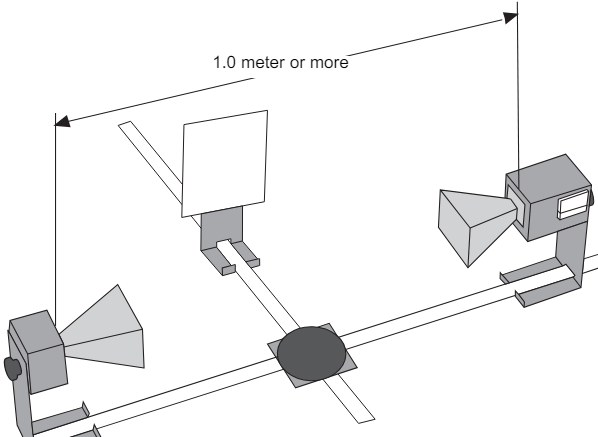
\includegraphics[width = 0.5\textwidth]{LloydSetup.png}
	\caption{Setup sperimentale per interferometro Lloyd}
	\label{fig:setupLloyd}
\end{figure}

In questo modo si vengono a creare due fasci: il primo percorre una distanza $d$ in linea retta, mentre il secondo
percorre una distanza $2\ \sqrt[]{h^2 + (d/2)^2}$. Tale differenza di percorso porta a delle interferenze:
se la differenza di cammino ottico è un multiplo intero di $\lambda$ si ha interferenza costruttiva,
altrimenti si ha interferenza distruttiva.\\
\begin{figure}[h!]
	\centering
	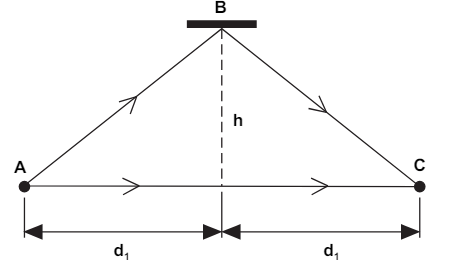
\includegraphics[width = 0.3\textwidth]{SchemaLloyd.png}
	\caption{Schema riassuntivo interferometro Lloyd}
	\label{fig:schemaLloyd}
\end{figure}

Al fine di misurare la lunghezza d'onda del fascio microonde, abbiamo seguito le istruzioni fornite dal manuale
Pasco e abbiamo variato la distanza $h$ alla ricerca di due minimi, una volta fissata la distanza $d$. 
Per poter eseguire un confronto sperimentale e non solo con il valore di $\lambda$ tabulato, 
abbiamo ripetuto la procedura per un'altra distanza $d$. \\
Come formula per il calcolo della lunghezza d'onda abbiamo utilizzato la \ref{eq:lloyd}, ricavata dalle relazioni 
geometriche che legano i cammini ottici e la differenza di fase tra i due fasci:
\begin{equation}
	\lambda = \frac{2h + 4\ \sqrt[]{(d/2)^2 + h^2}}{n}
	\label{eq:lloyd}
\end{equation}
Dalla prima misurazione abbiamo ottenuto due valori di $\lambda$ che abbiamo mediato, lo stesso abbiamo fatto per
la seconda misurazione.Come errori delle singole lunghezze d'onda abbiamo propagato gli errori a partire dall'equazione
\ref{eq:lloyd}, in seguito abbiamo propagato gli errori per la media. \\


\subsubsection{Analisi dati}
Riportiamo di seguito i dati raccolti durante l'esperienza e i risultati ottenuti.
Per la prima misurazione abbiamo scelto $d = 100 \pm 1$ cm, mentre per la seconda $d = 110 \pm 1$ cm. Abbiamo 
stimato le incertezze di 1 cm poichè sugli "horn" non erano ben segnalati i punti di emissione e di ricezione
dell'onda; non sapendo bene dove fossero localizzati abbiamo aumentato l'errore rispetto alla sensibilità 
della riga graduata.\\
In tabella \ref{tab:lloyd1} riportiamo i valori di $h$ e le intensità misurate per i minimi di interferenza,
in tabella \ref{tab:lloyd2} riportiamo i valori di $h$ e le intensità misurate per i massimi di interferenza.\\
Come valore $\lambda_1$ abbiamo ottenuto $2.86 \pm 0.07$ cm, mentre per $\lambda_2$ abbiamo ottenuto $2.85 \pm 0.06$ cm.\\
Abbiamo confrontato i valori ottenuti con il valore tabulato di $\lambda = 2.85$ cm, ottenendo:
\begin{enumerate}
	\item Distanza in deviazioni standard tra $\lambda_1$ e $\lambda_{tab}$: $0.11 \sigma$
	\item Distanza in deviazioni standard tra $\lambda_2$ e $\lambda_{tab}$: $0.08 \sigma$
	\item Distanza in deviazioni standard tra $\lambda_1$ e $\lambda_2$: $0.03 \sigma$
\end{enumerate}
L'ultimo punto è stato calcolato per verificare la coerenza tra i due valori di $\lambda$ ottenuti.\\

\subsubsection{Conclusioni}
Dai risultati ottenuti possiamo concludere che la lunghezza d'onda delle microonde calcolata tramite interferometro
di Lloyd è compatibile con il valore tabulato.
Al di là della misura della lunghezza d'onda tramite interferenza, questa sezione ci ha permesso di verificare
sperimentalmente un'ipotesi che spiega problemi verificatisi in altre sezioni: l'interferenza per riflessione 
delle microonde. Ogniqualvolta un esperimento richieda la rotazione del ricevitore, si possono considerare effetti 
di interferenza alla Lloyd, poichè, per angoli in cui ricevitore e emettitore sono sempre più vicini, 
si può modelizzare il sistema come un interferometro di Lloyd. Infatti l'interferenza alla Lloyd si ottiene 
quando un materiale che abbia proprietà riflettenti viene avvicinato all'apparecchiatura, portandoci a 
considerare questo effetto di interferenza in tutte le sezioni in cui ci troviamo a ruotare il ricevitore.\\

\subsection{Interferometro di Michelson}
In questa seconda esperienza sull'interferenza di onde abbiamo deciso di riprodurre una versione del note esperiemento di 
interferometria di Michelson e Morley.
\begin{figure}[h!]
	\centering
	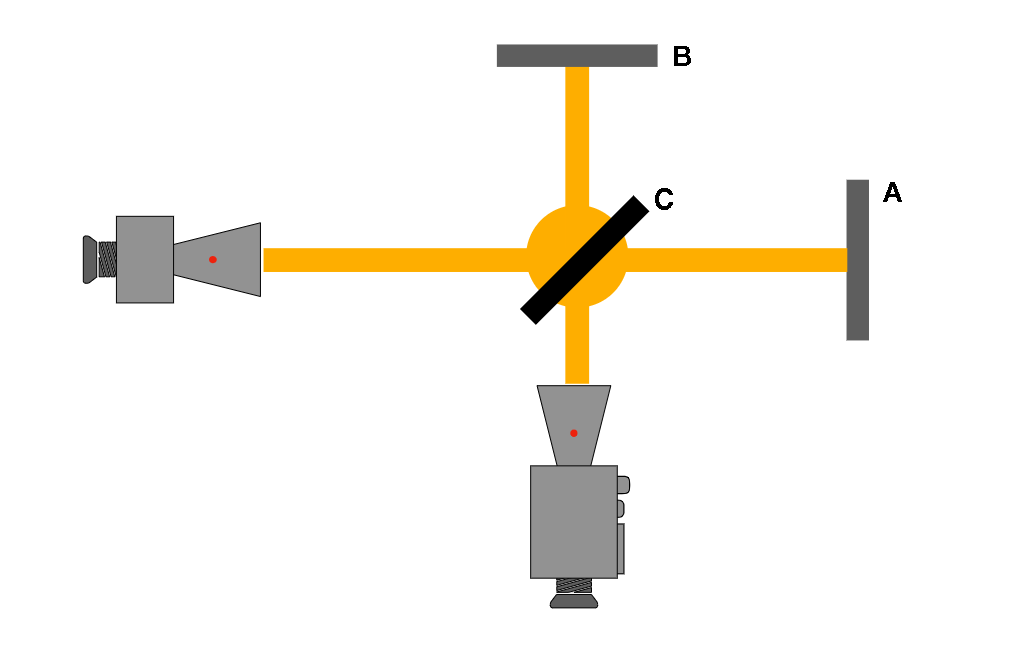
\includegraphics[width = 0.4\textwidth]{MichelsonSetup.png}
	\caption{Setup esperimento Michelson e Morley}
	\label{fig:GraficoBragg}
\end{figure}
Per questo setup abbiamo utilizzato due specchi riflettenti (placche metalliche)
che in figura sono segnati come B e A. Al centro abbiamo posizionato ad un angolo di 45 gradi una superficie semiriflettente.
Tenendo fermo uno dei due specchi e muovendo l'altro variamo il cammino ottico del raggio di luce che esce dall'emettitore e che si è diviso in due su C.
Percorrendo distanze diverse i due raggi quando ricongiungendosi ci aspettiamo creino la tipica figura a frange di interferenza.  
Se le due onde sono in fase quando arrivano al ricevitore ci attendiamo di misurare un massimo ogni $\lambda/2$ dove lambda è la lunghezza d'onda del raggio divisa per due dato che 
ogni onda passa due volte tra lo specchio e la superficie semiriflettente.

\subsubsection{Analisi Dati Michelson}
In questa sezione elenchiamo i risultati ottenuti dalle misure sperimentali.
Come suggerito dalla scheda e dal manuale Pasco, abbiamo deciso di spostare lo specchio A. Prima di tutto ci siamo posizionati attorno ad un
massimo del segnale (picco di voltaggio sempre con multimetro palmare), successivamente abbiamo allontanato lo specchio A attraversando 10 minimi. Una volta ritrovato un massimo ci siamo segnati tale nuova posizione.
\begin{enumerate}
	\item Posizione iniziale $x1 =(38.7 \pm0.2)$ cm
	\item Voltaggio iniziale $\Delta V1 = (0.82\pm0.02)$ V 
	\item Posizione finale $x2 =(24.5 \pm0.2)$cm
	\item Voltaggio finale $\Delta V2 = (0.87\pm0.02)$V
\end{enumerate}
Ripetendo le misure cambiando la distanza:
\begin{enumerate}
	\item Posizione iniziale $x1 =(43.0\pm0.2)$ cm
	\item Voltaggio iniziale $\Delta V1 = (1.1\pm0.02)$ V 
	\item Posizione finale $x2 =(28.8\pm0.2)$cm
	\item Voltaggio finale $\Delta V2 = (0.83\pm0.02)$V
\end{enumerate}
Infine di nuovo cambiando la distanza inziale:
\begin{enumerate}
	\item Posizione iniziale $x1 =(34.4\pm0.2)$ cm
	\item Voltaggio iniziale $\Delta V1 = (0.83\pm0.02)$ V 
	\item Posizione finale $x2 =(20.1\pm0.2)$cm
	\item Voltaggio finale $\Delta V2 = (0.86\pm0.02)$V
\end{enumerate}
Da queste misure abbiamo estrapolato una stima del valore della lunghezza d'onda, secondo la seguente relazione:
$$ \lambda = \frac{2\Delta x}{n} $$ 
Facendo una media delle tre misure e utilizzando la formula di propagazione degli errori abbiamo stimato:
$$\lambda_\text{mis} = (2.85 \pm0.01)\text{cm}$$
\subsubsection{Conclusioni Michelson e Morley}
Oltre ad aver effettivamente verificato la posizione dei massimi trovarsi ad una distanza pari a $\lambda/2$, 
il valore ottenuto per la stima della lunghezza d'onda è perfettamente in linea con il valore suggerito dal manuale Pasco.
Questo metodo sembra quello che ha restituito la misura più accurata di $\lambda$. Riportiamo in seguito un altro metodo per la stima 
della lunghezza d'onda sempre dalla raccolta dati:
\begin{figure}[h!]
	\centering
	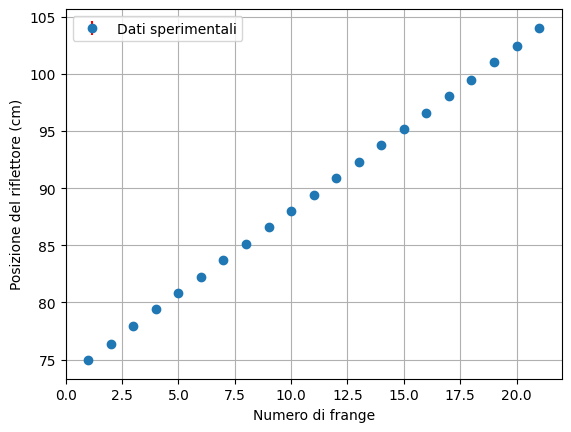
\includegraphics[width = 0.6\textwidth]{MichelsonGrafico.png}
	\caption{Setup esperimento Michelson e Morley}
	\label{fig:GraficoBragg2}
\end{figure}

Graficando il numero di frange oltrepassate rispetto alla posizione dello specchio A riflettente otteniamo una retta,
il cui coefficiente rappresenta mezza lunghezza d'onda. Fittando i nostri dati con un modello lineare abbiamo ottenuto:
\begin{enumerate}
	\item Stima coeff retta = $(1.44\pm0.004)$ cm
	\item Stima lunghezza d'onda $ \lambda = (2.89\pm0.01)$ cm
	\item Chi-quadro ridotto $\widetilde{\chi}^2 = 0.2$
\end{enumerate}

\newpage
\section{Diffrazione di Bragg}
In quest'ultima parte dell'esperienza abbiamo cercato di riprodurre a livello macroscopico 
una tecnica per "l'imaging" di piani atomici in cristalli reticolari. Per farlo abbiamo utilizzato come modello per il reticolo cristallino, un cubo di ethafoam 
contenente delle sferette di metallo di circa $10$mm. Queste sferette allo stesso modo della loro controparte microscopica (atomi in un normale reticolo) diffondono un fascio incidente e in base alla distanza d dei "piani atomici" producono figure di interferza.
Lo scopo di questa tecnica è quello di ricavare dallo studio delle figure di interferenza (massimi e minimi) la configurazione geometrica del cubo e in particolare trovare la distanza d tra i piani.
Di seguito alleghiamo delle figure rappresentative per la configurazione dell'esperimento.
\begin{figure}[h!]
	\centering
	\begin{subfigure}[b]{0.48\textwidth} % Adjust the width as needed
		\centering
		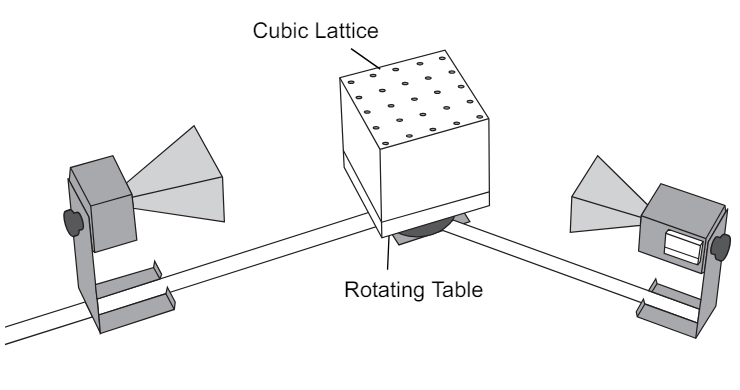
\includegraphics[width=\textwidth]{setup_bragg.png}
		\caption{Setup diffrazione Bragg}
		\label{fig:Setup Bragg}
	\end{subfigure}
	\hfill % Add horizontal space between the subfigures
	\begin{subfigure}[b]{0.3\textwidth} % Adjust the width as needed
		\centering
		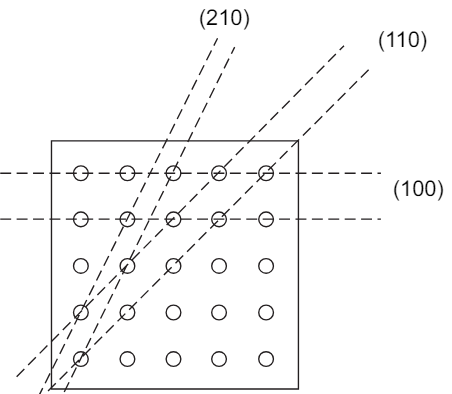
\includegraphics[width=\textwidth]{piani_bragg.png}
		\caption{Piani di incidenza}
		\label{fig:Piani di Bragg}
	\end{subfigure}
	\caption{Setup diffrazione di Bragg}
\end{figure}

Per il campionamento delle misure, abbiamo posizionato emettitore e ricevitore come in figura \ref{fig:Setup Bragg}
e abbiamo deciso di studiare il fascio in relazione al piano di incideza $(100)$. Per questi indici di Miller dei piani cristallini abbiamo $n=1$, ovvero un solo piano attraversato lungo direzione del fascio.
In questo caso dunque la condizione per cui si verificherà la diffrazione dell'onda incidente:
\begin{equation}
	n \lambda = 2dsin(\theta) \quad ,n=1
	\label{eq:Legge Bragg}
\end{equation}
In questa relazione, d rappresenta la nostra incognita, lambda è la lunghezza d'onda nota e $\theta$ rappresenta
l'angolo tra il fascio incidente e la superficie del cubo secondo la seguente figura 
\begin{figure}[h!]
    \centering
    \begin{subfigure}[b]{0.28\textwidth}
        \centering
        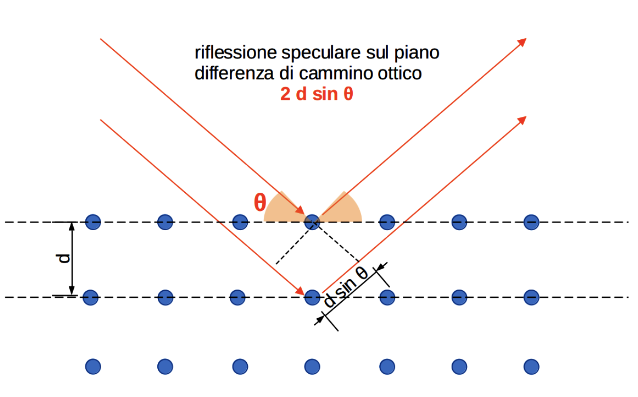
\includegraphics[width=\textwidth]{diffrazione_bragg.png}
        \caption{Riflessione su reticolo}
        \label{fig:Reticolo Bragg}
    \end{subfigure}
    \hspace{0.3\textwidth} 
    \begin{subfigure}[b]{0.28\textwidth}
        \centering
        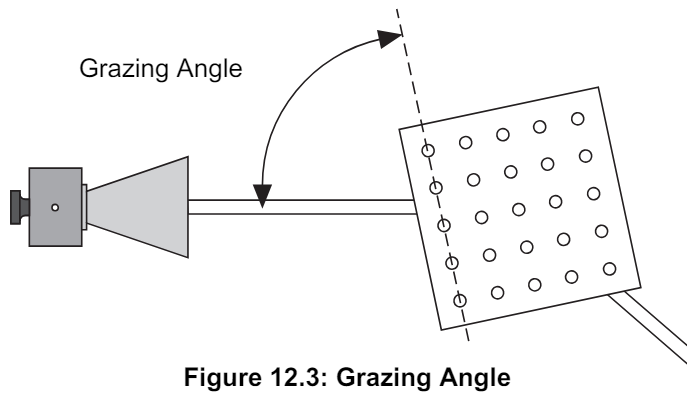
\includegraphics[width=\textwidth]{angolo_bragg.png}
        \caption{Angolo di incidenza}
        \label{fig:Angolo Bragg}
    \end{subfigure}
    \caption{Diffrazione di Bragg e angolo}
    \label{fig:combined_figures}
\end{figure}

\newpage
\subsection{Analisi Dati Bragg}
In questa sezione riportiamo le misure effettuate per la verifica della legge di Bragg (Eq. \ref{eq:Legge Bragg}). Dopo aver acceso e posizionato l'emettitore di fronte al ricevitore come nel setup, abbiamo iniziato a ruotare il cubo di $\theta = 2\text{°}$ per volta e di conseguenza il braccio che sosteneva il ricevitore di $\theta' = 2\theta = 4\text{°}$.
Ripetendo questa procedura abbiamo segnato per ogni angolo di rotazione, il valore dell'intensità del segnale catturato dal ricevitore.
Graficando gli angoli di incidenza con il voltaggio del ricevitore otteniamo: 
\begin{figure}[h!]
	\centering
	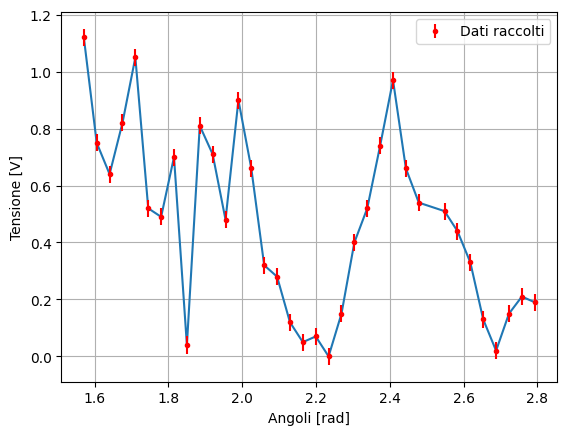
\includegraphics[width = 0.6\textwidth]{Grafico1_bragg.png}
	\caption{Grafico angoli-intesità per Bragg}
	\label{fig:GraficoBragg3}
\end{figure}

La regione di interesse nel grafico è quella del picco attorno a $\theta=2.4$. I primi picchi rappresentano probabilmente riflessioni da altri piani rispetto a quello sotto nostra analisi (100).
Ci aspettiamo che la relazione di Bragg si verifichi quando:
$$ \lambda = 2dsin(\theta) $$
riarrangiando i termini in questa equazione ci aspettiamo di trovare un picco nel segnale,il quale rappresenta un massimo del raggio difratto, attorno a quest'angolo:
$$ \theta_\text{atteso} = arcsin(\frac{\lambda}{2d}) = arcsin(\frac{2.85\text{cm}}{2\times(\text{insert real d})}) =  $$ 
Dal grafico delle nostre misure abbiamo notato un picco per $$\theta_\text{mis} = (138 \pm1)\text{°} = (2.40 \pm0.1)\text{ rad}$$
Da questo valore possiamo trovare una stima per la distanza tra i piani atomici.
Inserendo l'angolo e propagando l'errore secondo questa formula: 
$$ d = \frac{\lambda}{2sin(\theta_\text{mis})} \quad \delta d = \sqrt{\left( \frac{\partial d}{\partial \theta} \right)^2 (\delta \theta_\text{mis})^2} $$ 
otteniamo una stima per la distanza: $$ d_\text{stima} = (2.13 \pm0.3) \text{cm} $$ 	
Confrontandola con la vera distanza: $$ d_\text{true} = ( \pm) \text{cm} $$ 

Abbiamo inoltre provato ad eseguire un fit con due modelli differenti per estrapolare un'ulteriore stima dell'angolo di Bragg.
Due modelli alternativi che spesso vengono comunemente utilizzati per descrivere picchi in esperimenti simili sono: gaussiano, picchi con code brevi e il lorentziano per picchi con code più importanti.
Le due forme funzionali sono
\begin{equation}
	y = A \exp\left(-\frac{(x - \mu)^2}{2\sigma^2}\right)
	\end{equation}
	
	\begin{equation}
	y = A \frac{w^2}{(x - x_0)^2 + w^2}
	\end{equation}
Di seguito riportiamo un grafico dei fit effettuati per questi due modelli, per quanto riguarda le incertezze:
\begin{enumerate}
	\item Incertezza sull'angolo è di $\delta\theta= 1$ grado dettata da sensibilità goniometro.
	\item Incertezza sull'intensità abbiamo scelto $\delta V = 0.05 V$ dettata sia dalla sensibilià del palmare che da noise nelle misure.
\end{enumerate}
\begin{figure}[h!]
	\centering
	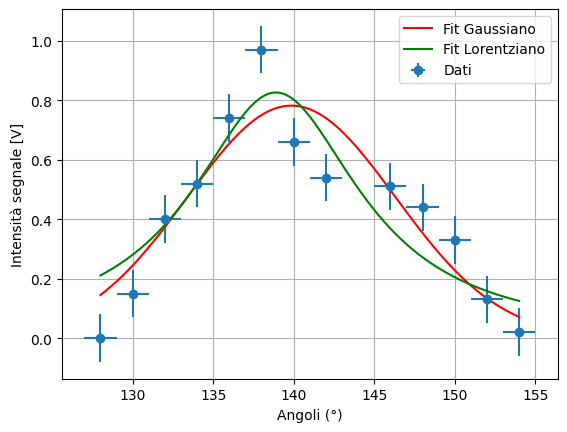
\includegraphics[width = 0.7\textwidth]{graf_bragg.png}
	\caption{Grafico angoli-intesità per Bragg}
	\label{fig:GraficoBragg4}
\end{figure}

\subsection{Conclusioni Bragg}
Di seguito riportiamo i risultati ottenuti dal fit e in generale da questa parte dell'esperienza.
Anche se realtivamente approssimativi i fit hanno restituito come angolo di Bragg un valore molto vicino a $138$
e in particolare il chi-quadro ridotto è più basso per il modello gaussiano, il che sottolinea che si tratta di un segnale dove il picco è più importante delle code.
In generale analizzando la differenza tra la distanza attesa e quella estrapolata dalle misure possiamo concludere che quel picco 
rappressenta effettivamente il segnale del raggio diffratto. Ricordiamo inoltre che tali misure sono state effettuate per il piano di incidenza denotato da 
(100).

\begin{table}[h!]
    \centering
    \caption{Riassunto dei risultati dei fit}
    \label{tab:fit_results}
    \begin{tabular}{|l|c|c|}
        \hline
        \textbf{Modello} & \textbf{Parametro} & \textbf{Valore} \\
        \hline
        Gaussiano & $A$ & $0.782 \pm 0.070$ \\
                  & $\mu$ & $139.861 \pm 0.669$ \\
                  & $\sigma$ & $6.463 \pm 0.667$ \\
        \hline
        Lorentziano & $A$ & $0.826 \pm 0.093$ \\
                    & $x_0$ & $138.898 \pm 0.767$ \\
                    & $w$ & $6.379 \pm 1.149$ \\
        \hline
        Chi-quadro ridotto & Gaussiano & 2.528 \\
                            & Lorentziano & 3.166 \\
        \hline
    \end{tabular}
\end{table}
\newpage
\section{Tabelle misurazioni}

\begin{table}[h!]
	\centering
	\caption{Lloyd: prima misura}
	\label{tab:lloyd1}
	\begin{tabular}{|c|c|}
		\hline
		$h$ [cm] & $I$ [V] \\
		\hline
		9.9      & 1.64    \\
		16.9     & 1.7     \\
		\hline
	\end{tabular}
\end{table}

\begin{table}[h!]
	\centering
	\caption{Lloyd: seconda misura}
	\label{tab:lloyd2}
	\begin{tabular}{|c|c|}
		\hline
		$h$ [cm] & $I$ [V] \\
		\hline
		10.9     & 1.40    \\
		17.2     & 1.5     \\
		\hline
	\end{tabular}
\end{table}

\newpage
\section{Grafici Brewster}
Sono riportati i grafici che non tornano con l'andamento atteso.

\begin{figure}[h!]
	\centering
	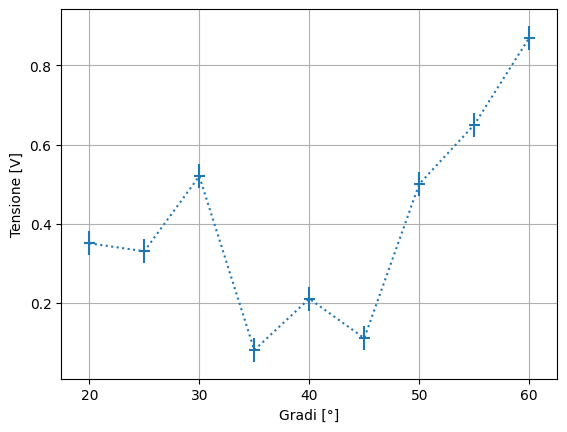
\includegraphics[width = 0.6\textwidth]{riflesso1.png}
	\caption{Intensità del raggio riflesso - prima giornata}
	\label{fig:riflesso1}
\end{figure}

\begin{figure}[h!]
	\centering
	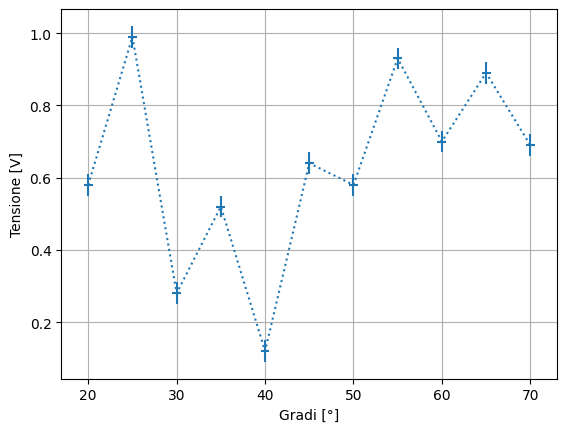
\includegraphics[width = 0.6\textwidth]{riflesso2.png}
	\caption{Intensità del raggio riflesso - seconda giornata}
	\label{fig:riflesso2}
\end{figure}

\end{document}
